To check the resulting analytical model, we calculated the values of the complex refractive index $m$, which correspond to the previously obtained conditions for the resonance electron density $n_{el}$ at $\lambda_{10} = 83$ nm, $ka = 0.7$: $m = 1.851i$ (\ref{m2_resonance}). The complex refractive index is purely imaginary, since the collision coefficient $v_e$ in the case under consideration is somewhat lower than the harmonic frequency, so the interaction can be considered collisionless~\cite{andreev_lecz}.

For this case, the scattered electric field (\ref{E_s_sph}) was calculated for $\lambda = \lambda_{L}$ and $\lambda = \lambda_{10}$ in order to compare the resonant and nonresonant cases. It can be seen that in the resonance case (\ref{ka0.7:b}) the scattered field is a diverging spherical wave, the field amplitude in the vicinity of the cluster is much higher than in the absence of resonance (\ref{ka0.7:a}), where Scattered waves as such are practically not observed, which indicates that the incident wave in the nonresonant case practically does not interact with the cluster.

    \begin{tikzfigure}
        \subcaptionbox{$\lambda = \lambda_{L} = 830$ nm.}{
            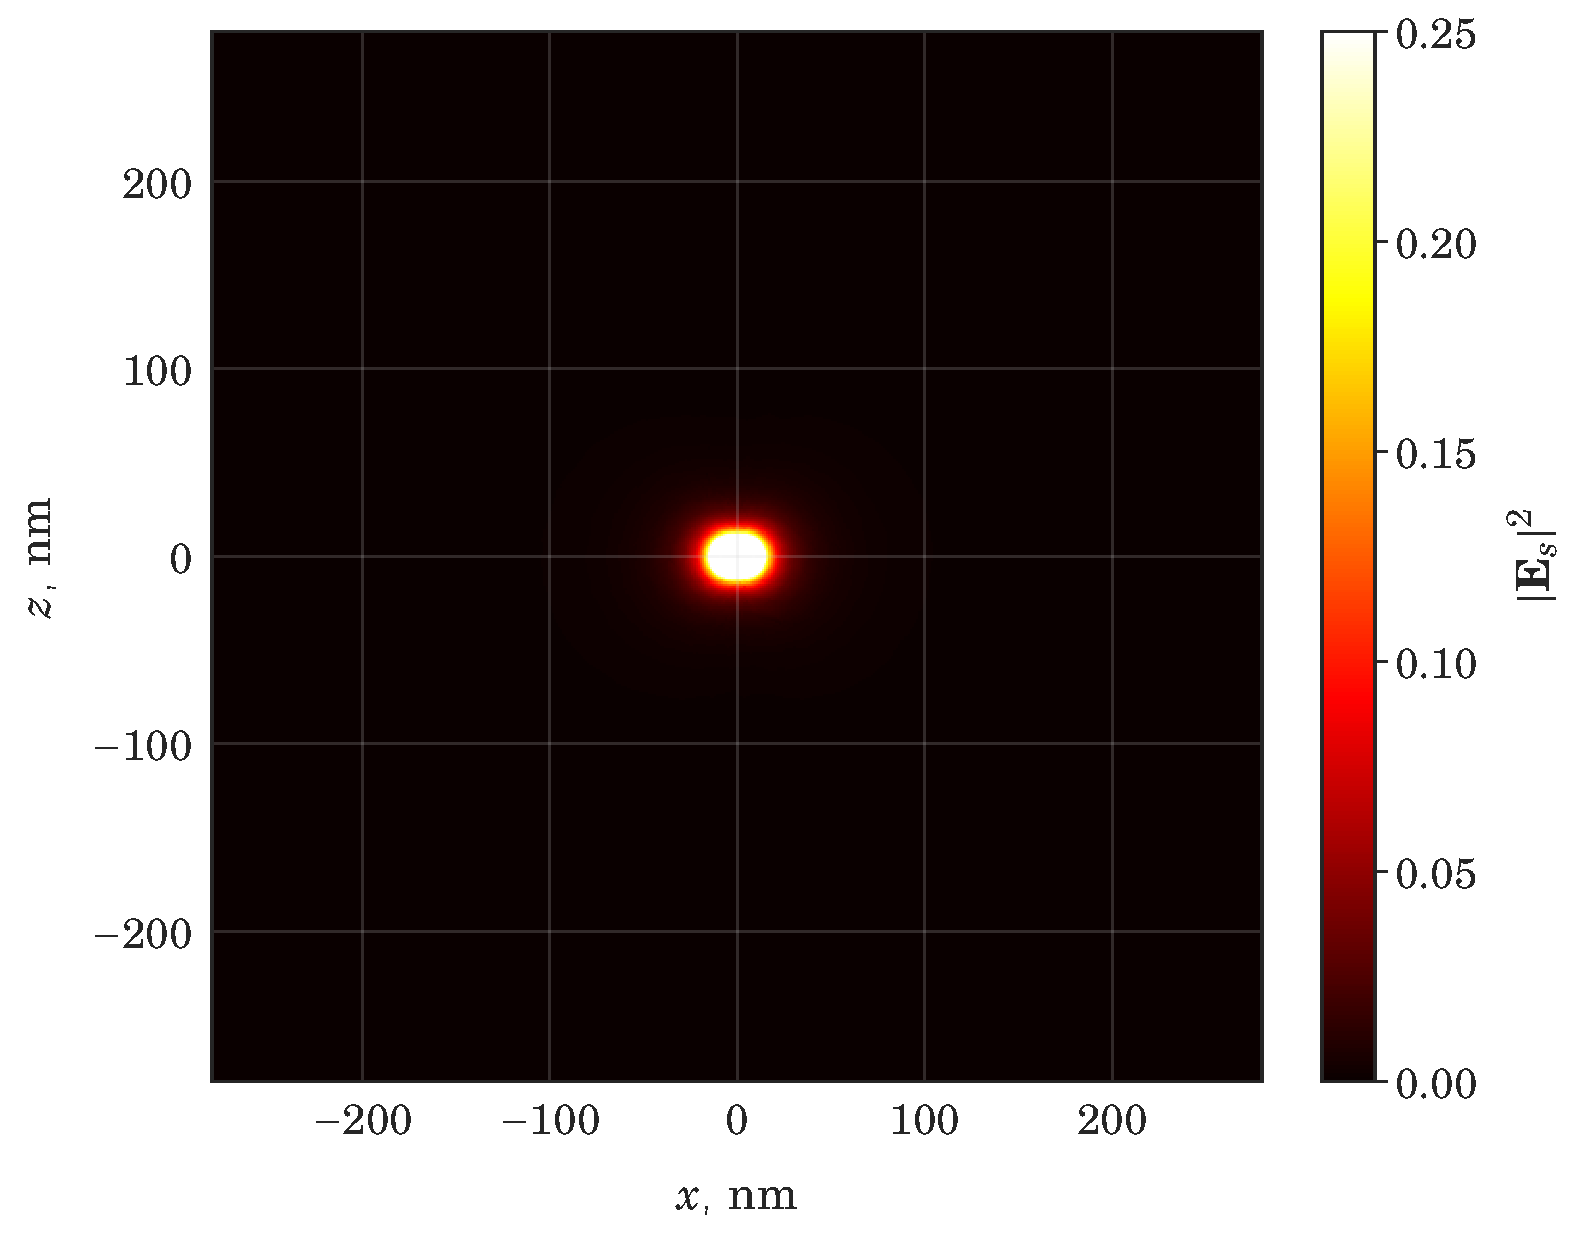
\includegraphics[width=0.45\linewidth]{../components/img/mph_new/es_ka0.7_1harm}
        }
        \hfil
        \subcaptionbox{$\lambda = \lambda_{10} = 83$ nm.}{
            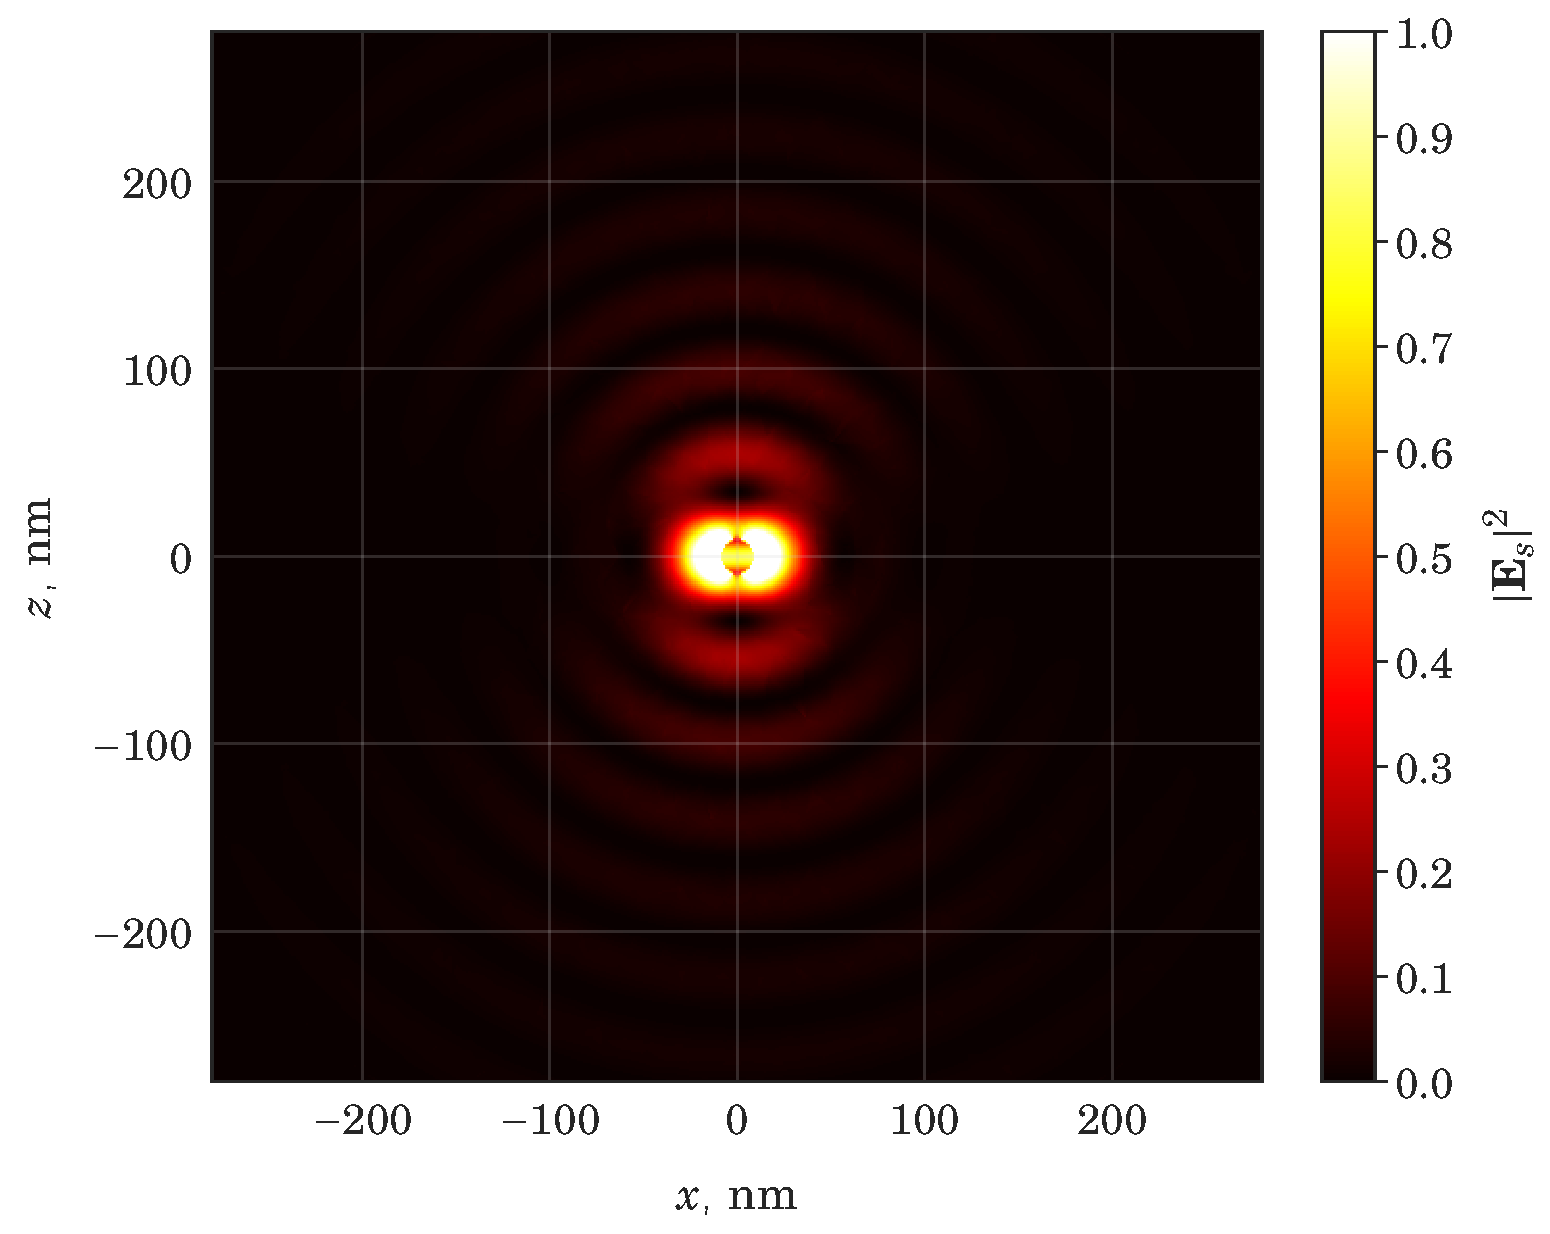
\includegraphics[width=0.45\linewidth]{../components/img/mph_new/es_ka0.7_10harm}
        }
        \label{ka0.7:image}\caption{$ka = 0.7$ ($a \approx 8.9$ nm); $|\vectbf{E}{s}|^2$ in the plane of polarization of the incident wave.}
    \end{tikzfigure}

    % \begin{figure}[H]
    %     \subimgtwo[components/img/mph_new/es_ka0.7_1harm]{$\lambda = \lambda_{L} = 830$ nm.}{ka0.7:a}{0.4\textwidth}
    %     \hfil
    %     \subimgtwo[components/img/mph_new/es_ka0.7_10harm]{$\lambda = \lambda_{10} = 83$ nm.}{ka0.7:b}{0.4\textwidth}
    %     \caption{$ka = 0.7$ ($a \approx 8.9$ nm); $|\vectbf{E}{s}|^2$ в плоскости поляризации падающей волны.}\label{ka0.7:image}
    % \end{figure}

    % \begin{figure}[H]
    %     \subimgtwo[components/img/mph_new/es_ka1.7_10harm]{Рассеяние кластером.}{10h_ka0.7:a}{0.4\textwidth}
    %     \hfil
    %     \subimgtwo[components/img/external/oe-28_screen_single.jpg]{Рассеяние наноцилиндром~\cite{andreev_lecz}.}{10h_ka0.7:b}{0.39\textwidth}
    %     \caption{$ka = 1.7$ ($a \approx 22.5$ nm), $\lambda = \lambda_{10} = 83$ нм; $|\vectbf{E}{s}|^2$ построено в плоскости поляризации падающей волны. Качественное сравнение для такого же значения $ka$ в случае цилиндров (б) --- падающая волна распространяется справа налево (противоположно направлению оси $x$), $y$-поляризована.}\label{10h_ka0.7:image}
    % \end{figure}

% Дополительно был смоделирован случай $ka = 1.7$ (\ref{10h_ka0.7:a}) и сравнён с аналогичной ситуацией для одиночного наноцилиндра~\cite{andreev_lecz} (\ref{10h_ka0.7:b}). Видно, что общие направления рассеянного поля сохраняются, видны слабые боковые порядки с углами отклонения, близкими к $90^\circ$ относительно направления падающей волны, что сходно с случаем цилиндрической симметрии. Различия в амплитуде рассеянных волн связаны с принципиальными отличиями в геометрии цилиндра и кластера. Наиболее интенсивное рассеяние наблюдается для направления, соответствующего направлению падающей волны в силу конструктивной интерференции, эффективность рассеяния в этом направлении порядка 5\%.